\documentclass{article}
\usepackage[utf8]{inputenc}
\usepackage{amssymb, amsmath, amsthm, amsfonts, cancel, hyperref, tikz, enumitem, forest, float}
\usetikzlibrary{arrows.meta}
\usetikzlibrary{positioning, shapes, arrows, bayesnet}
\usetikzlibrary{bayesnet}
\usepackage{array}
\usepackage{booktabs}
\usepackage[margin=0.75in]{geometry}
\newcommand{\brac}[1]{\left\{ #1\right\}}
\newcommand{\un}[1]{\underline{#1}}
\newcommand{\p}[1]{\left({#1}\right)}
\setlength{\parskip}{1em}
\begin{document}
\title{Final Project}
\date{}
\author{
\textbf{Tri-An Nguyen}\\
RUID: 221008675\\
netid: tdn39
\and
\textbf{Sebastian Massella}\\
RUID: 207000623\\
netid: sxm4
\and
\textbf{Arjan Abazovic}\\
RUID: 209009268\\
netid: aa2386}
\maketitle 

\section*{Introduction}
In this project, we implement the perception algorithm, a three-layer neural network, and a three-layer neural network using PyTorch to detect faces and classify digits. We train these algorithms first on 10\% of the training data, then 20\%, up to 100\%, to investigate the results as a function of the percentage of training data used. We compare the performance of the algorithms on the test data, and report the average training time and the average test accuracy (and standard deviation) as a function of the percentage of training data used.
\section*{Data Preparation}
To extract the digit and face data from the given text images, we used the data processing code provided by UC Berkeley \url{https://ai.berkeley.edu/classification.html}. After loading the data from their corresponding files, we created digit and face data features. We chose straightforward features for both datasets by making each pixel a feature. For the digit train and test sets, we set the value of a pixel feature to 0 if the pixel is blank, 1 if the pixel is gray, and 2 if the pixel is black. Similarly, for the face train and test sets, we set the value of a pixel feature to 0 if the pixel is blank, and 1 if the pixel is an edge.

\section*{Perceptron Algorithm}
We trained the perceptron algorithm using a percentage of the training data (10\%, 20\%, ..., 100\%), 5 times each, to gather training time and test accuracy averages. Before inputting the training data into the algorithm to train, we randomly selected data samples. We implemented the perceptron algorithm by following the steps shown in the lecture. First, we initialized the weights to zero and the maximum epochs to 100, to give our simple algorithm enough time to train on relatively complex datasets. Then we went through every data point in the training data, computing the dot product between the weights and the data sample. If the product matches the label, we continue; if not, we update the weights accordingly. This process continues until we make a pass on the training data without making any updates, or the maximum number of epochs is reached. We evaluated the trained model on the test set. 

\noindent Below are plots showing average training time and test accuracy per percentage of training data for each dataset, followed by the output log.
\begin{figure}[H]
    \centering
    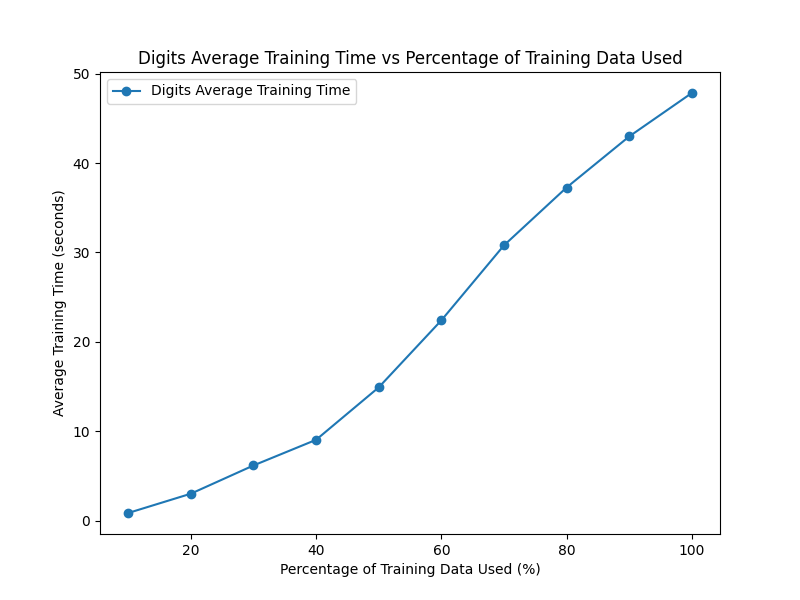
\includegraphics[width=.75\textwidth]{report/report_figures/perceptron_digits_time.png}
\end{figure}
\begin{figure}[H]
    \centering
    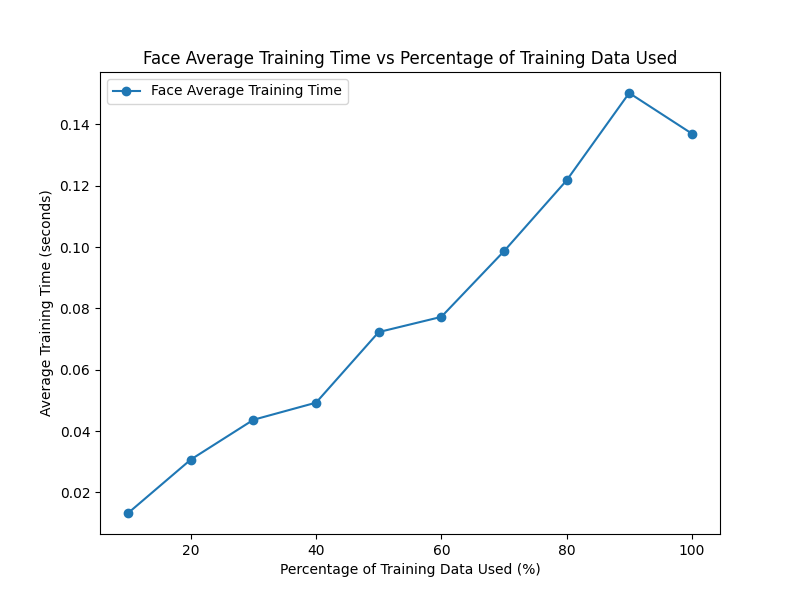
\includegraphics[width=.75\textwidth]{report/report_figures/perceptron_face_time.png}
\end{figure}
\begin{figure}[H]
    \centering
    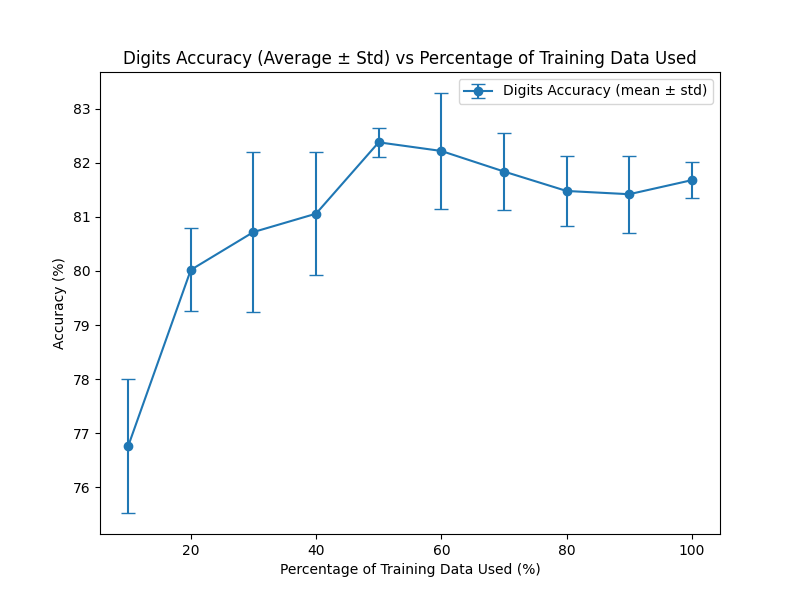
\includegraphics[width=.75\textwidth]{report/report_figures/perceptron_digits_acc.png}
\end{figure}
\begin{figure}[H]
    \centering
    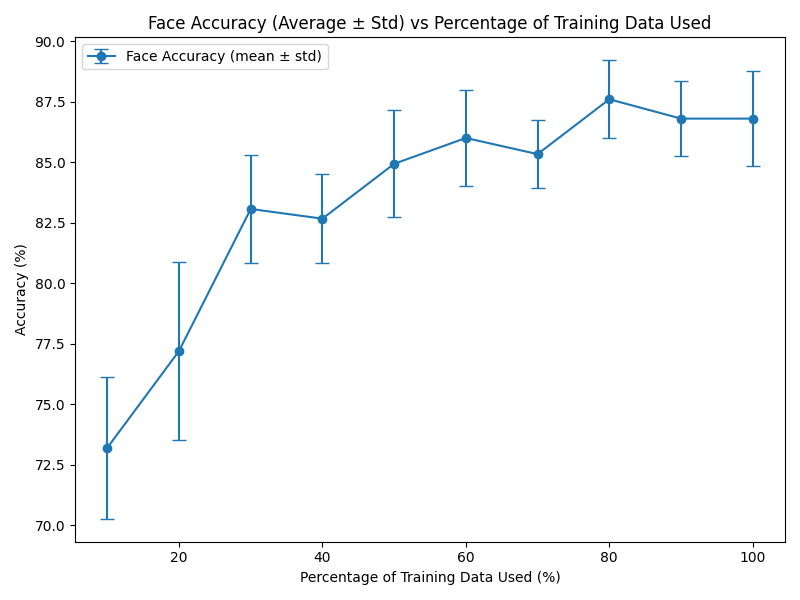
\includegraphics[width=.75\textwidth]{report/report_figures/perceptron_face_acc.png}
\end{figure}
\begin{figure}[H]
    \centering
    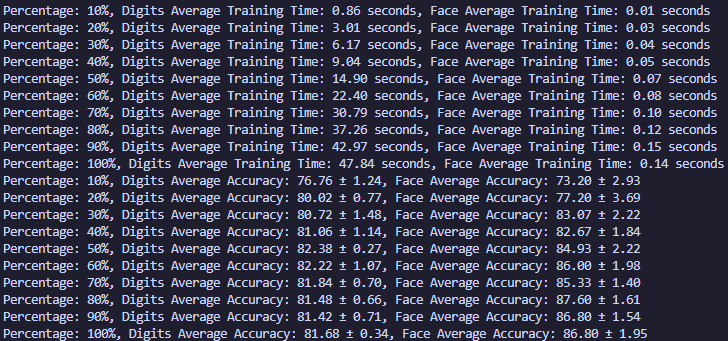
\includegraphics[width=.75 \textwidth]{report/report_figures/perceptron_output_log.png}
\end{figure}

\noindent Based on the average training time plots and output logs, the average training time for both datasets linearly increases with the percentage of data used. This is expected as the more training data, the more computational effort is required. The training time for the digits dataset is also much higher than the face dataset for the same percentage, which is also expected, as there is more training data for the digits dataset. 

\noindent Based on the average test accuracy plots and output logs, the test accuracy generally increases for both datasets; however, the digits dataset plateaus much quicker. The digits data accuracy increases to about 81\% using 40\% of the training data, and stays around 81\%-82\% accuracy for the rest of the training. The face data accuracy, on the other hand, increases throughout most of the training, only plateauing around 90\%-100\%. The output log shows that the standard deviation for both datasets generally decreases with the percentage of training data, which shows the accuracy is becoming more consistent. The face dataset's test accuracy is higher than the digit dataset after 30\% of the data is used. 

\section*{Three-layer Neural Network}
First, we defined our neural network class containing an input layer, two hidden layers, and an output layer, all as type \texttt{np.longdouble} to mitigate underflow. We used Sigmoid as the activation function and initialized the weights in the network using Xavier Initialization to help prevent vanishing gradients during training. We used 20 neurons in each hidden layer because it produced good results while keeping model complexity low. We also experimented with different values of L2 regularization and found 0.0 regularization to achieve the best results, as our model did not have an overfitting problem. We adjusted the learning rates to find the learning rate that balanced convergence speed and accuracy. We found the digits dataset worked well with a 0.5 learning rate, while the face dataset worked well with a 0.7 learning rate. 

\noindent We suspect the following reason for such high learning rates: due to the use of the sigmoid function, we encountered vanishing gradients as described above. So having a high learning rate enabled us to still learn and change the weights, even when the gradient was super small. Additionally, we set the learning rate for the digits dataset lower because there is more nuance as there are 10 output neurons.

\noindent We trained the neural network using a percentage of the training data (10\%, 20\%, ..., 100\%), 5 times each, to gather training time and test accuracy averages. Before inputting the training data into the model to train, we randomly selected data samples. We trained the digits dataset for 1000 epochs and the face dataset for 100 epochs. In each epoch, we manually computed the forward pass, the loss/cost, the backward pass, and updated the weights. Once training was completed, we evaluated the model on the test set. 

\noindent Below are plots showing average training time and test accuracy per percentage of training data for each dataset,
followed by the output log.

\begin{figure}[H]
    \centering
    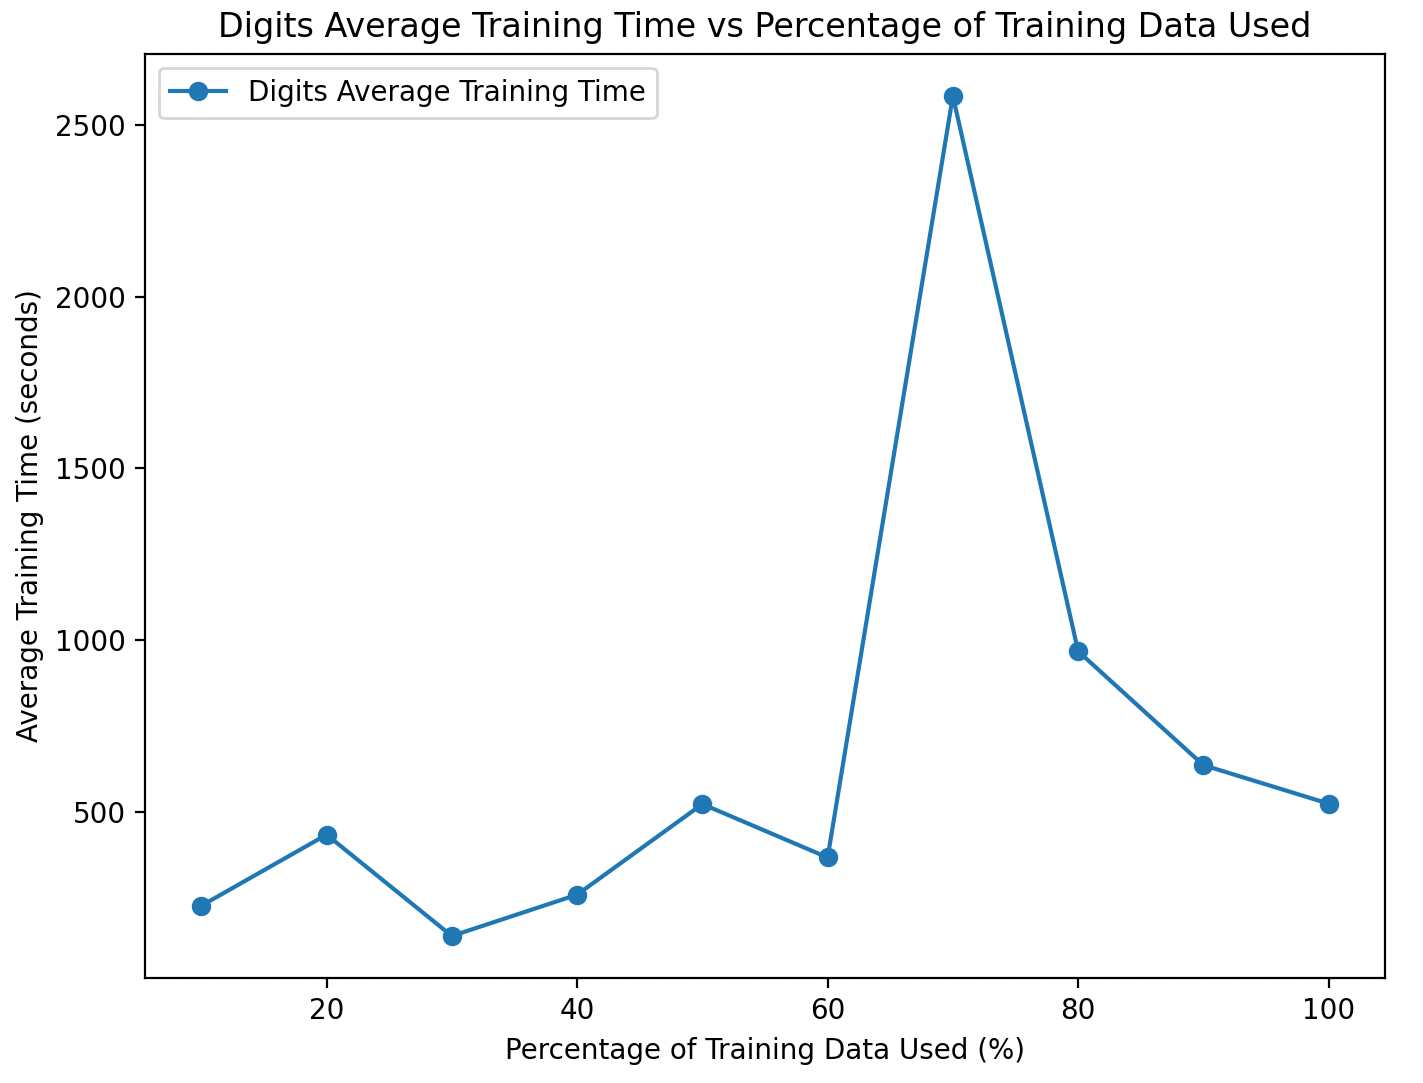
\includegraphics[width=.75\textwidth]{report/report_figures/nn_digits_time.png}
\end{figure}
\begin{figure}[H]
    \centering
    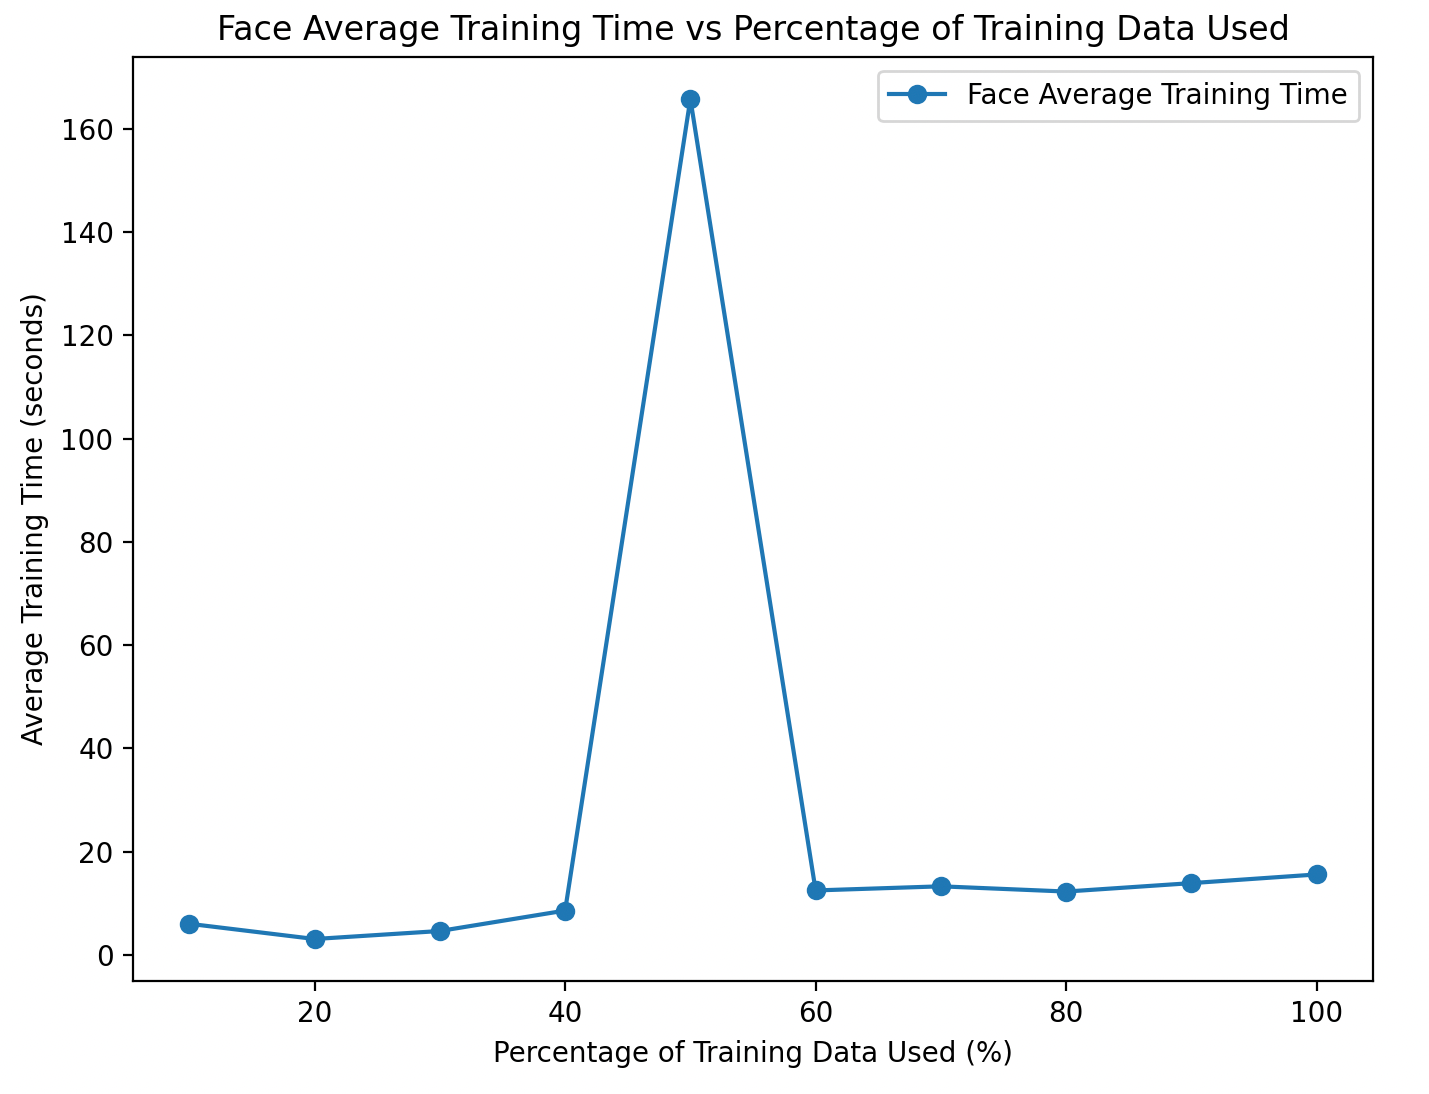
\includegraphics[width=.75\textwidth]{report/report_figures/nn_face_time.png}
\end{figure}
\begin{figure}[H]
    \centering
    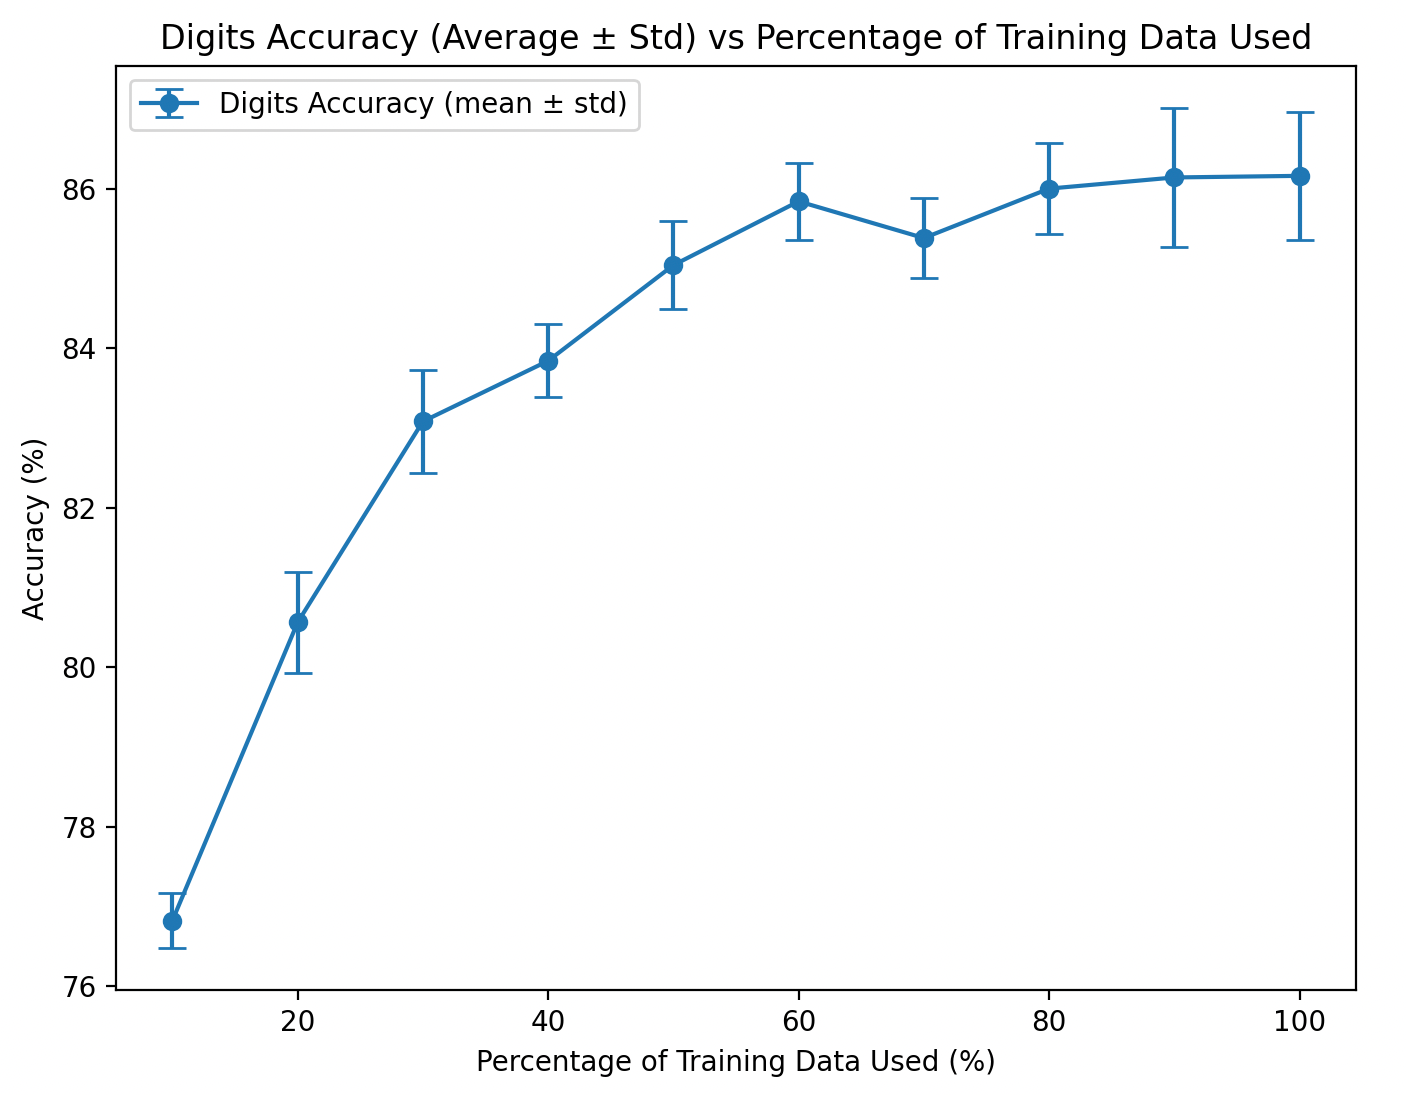
\includegraphics[width=.75\textwidth]{report/report_figures/nn_digits_acc.png}
\end{figure}
\begin{figure}[H]
    \centering
    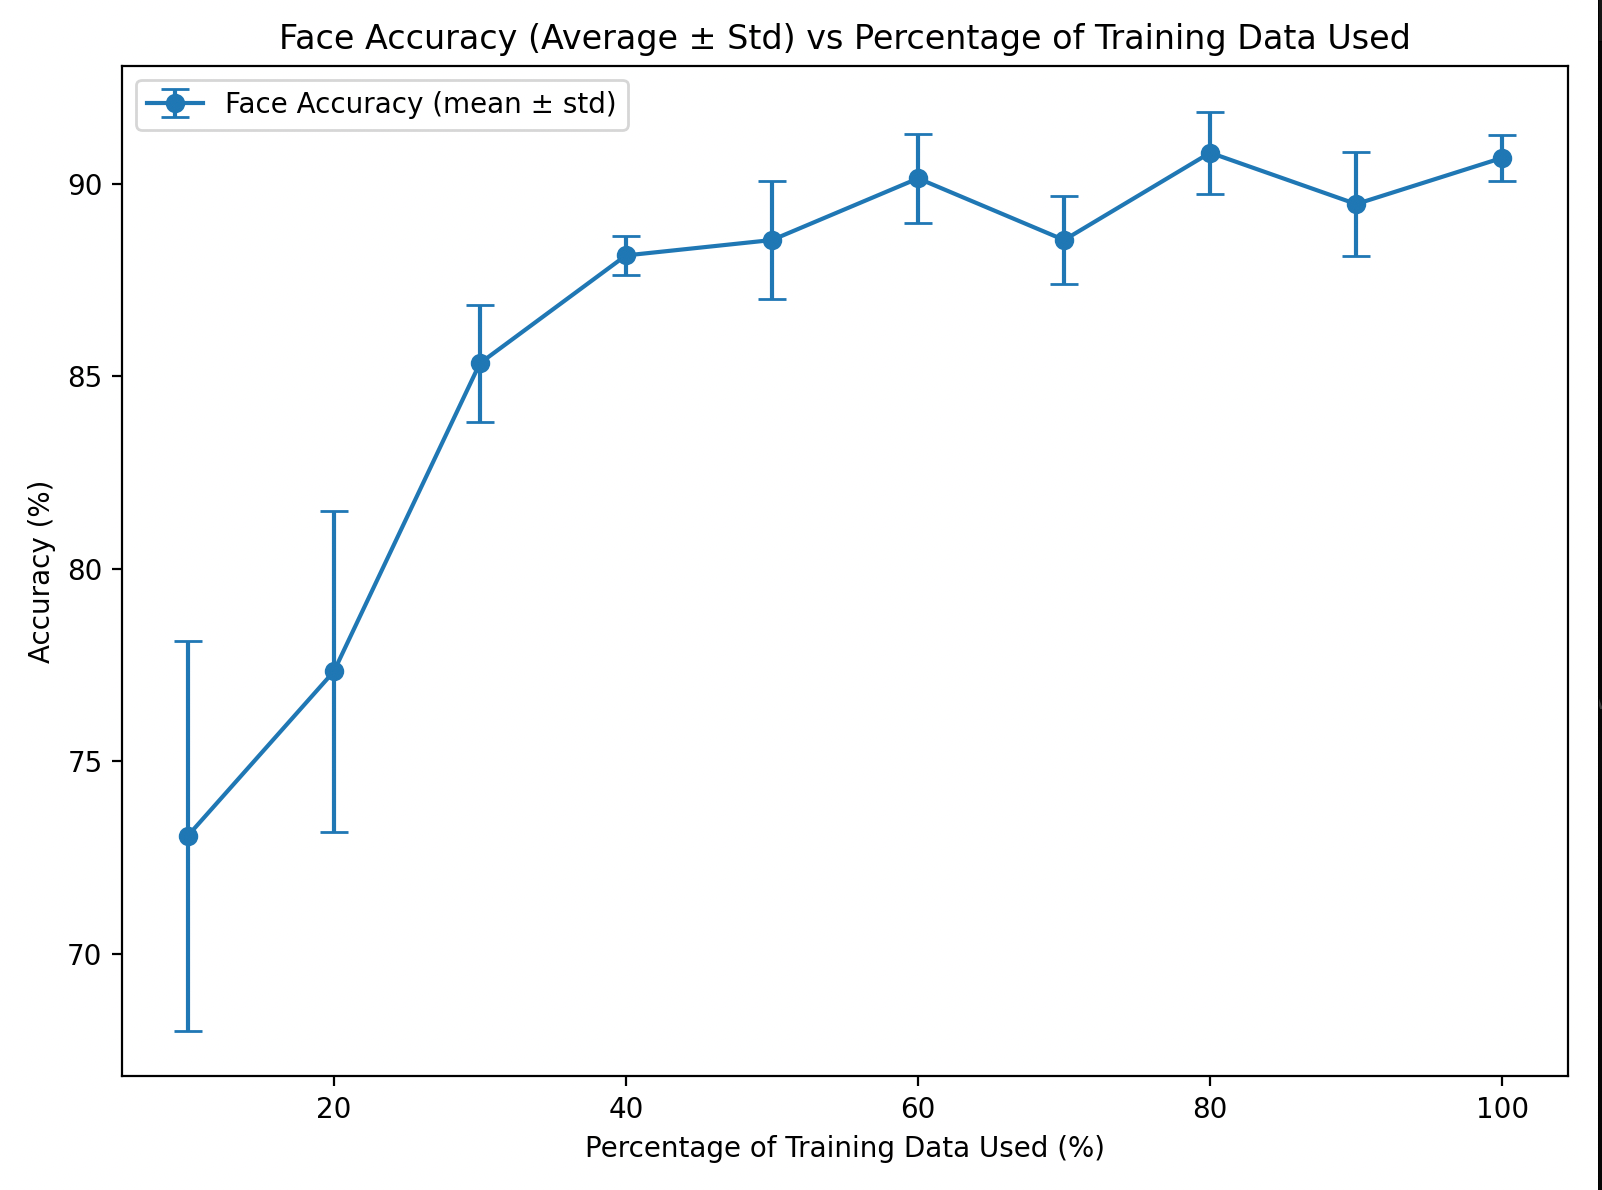
\includegraphics[width=.75\textwidth]{report/report_figures/nn_face_acc.png}
\end{figure}
\begin{figure}[H]
    \centering
    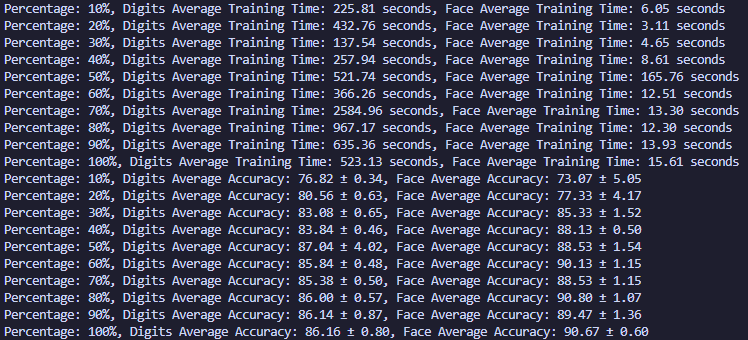
\includegraphics[width=.75 \textwidth]{report/report_figures/nn_output_log.png}
\end{figure}

\noindent Based on the average training time plots and output logs, the training time generally increases with the percentage of training data used, as expected. The training time for the digits dataset doesn't linearly increase, which could be for reasons such as vanishing gradients or the computer that was used for training. The face dataset does have that linear relationship between the training time and portion of training data used, besides the one spike. Also, the training for the digits dataset took significantly longer than the face dataset. To speed up training, the ReLU activation function could be used, which mitigates vanishing gradients. 

\noindent Based on the average test accuracy plots and output logs, the test accuracy generally increases with the percentage of training data used. For the digits dataset, the test accuracy increases but then begins to plateau around 80\%-100\%. The face dataset's test accuracy also increases, but then plateaus around 70\%-100\%. The standard deviation in accuracy is mostly below 1 for the digits dataset, showing consistency in accuracy. For the face dataset, the standard deviation starts large and then quickly decreases, indicating the accuracy is becoming more consistent with more data. The face detection task achieves higher accuracy than the digit recognition task past 20\% training data.

\section*{Three-layer Neural Network using PyTorch}
First, we defined our neural network class containing an input layer, two hidden layers, and an output layer. We experimented with different numbers of neurons in each hidden layer, such as \{100, 100\}, \{100, 50\}, \{250, 250\}, in the first and second layers, respectively. We found that the different numbers of neurons produced similar results; therefore, we went with \{100, 100\} for simplicity. The number of output neurons depends on the dataset. For the digits dataset, the output was of size 10, corresponding to the 10 digits, whereas, for the face dataset, the output size was 2, corresponding to detecting a face or not.

\noindent For the activation function, we chose Sigmoid, and for the loss function, we used cross-entropy loss. We used stochastic gradient descent as the optimizer with a 0.1 learning rate. We experimented with different learning rates, such as \{0.1, 0.01, 0.001\}, and found 0.1 significantly performs the best in speed and accuracy, which aligns with the fact that SGD works well with larger learning rates. We also experimented with different amounts of L2 regularization, such as \{0.0, 0.01, 0.001\}, and found that 0.0 L2 regularization performed the best in accuracy and significantly in training time.

\noindent We trained the model using a percentage of the training data (10\%, 20\%, ..., 100\%), 5 times each, to gather training time and test accuracy averages. Before inputting the training data into the model to train, we randomly select data samples. We transform the training data into tensors, then train the neural network for 10 epochs. The training process includes putting the data sample through the model and getting the output, calculating the loss, computing the gradients, and then updating the weights. Once the model finished training, we evaluated it on the test data.

\noindent Below are plots showing average training time and test accuracy per percentage of training data for each dataset, followed by the output log.
\begin{figure}[H]
    \centering
    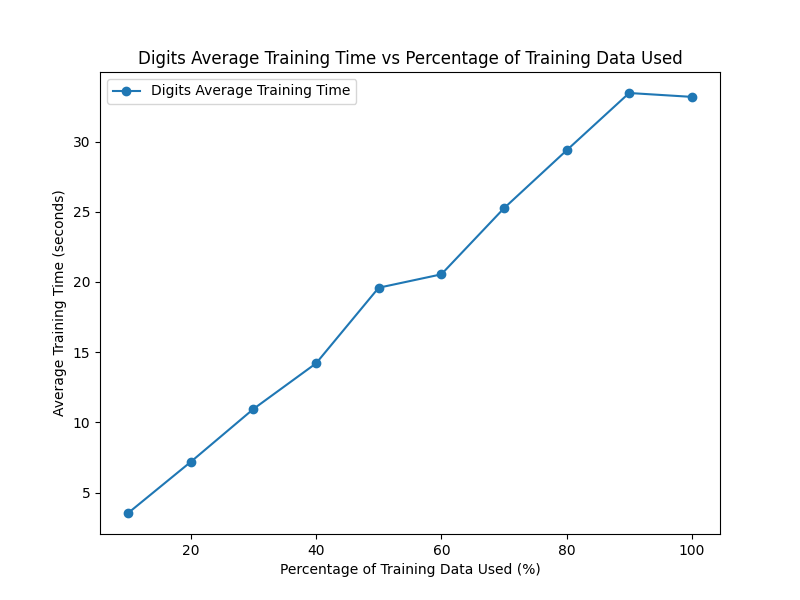
\includegraphics[width=.75\textwidth]{report/report_figures/pytorch_digits_time.png}
\end{figure}
\begin{figure}[H]
    \centering
    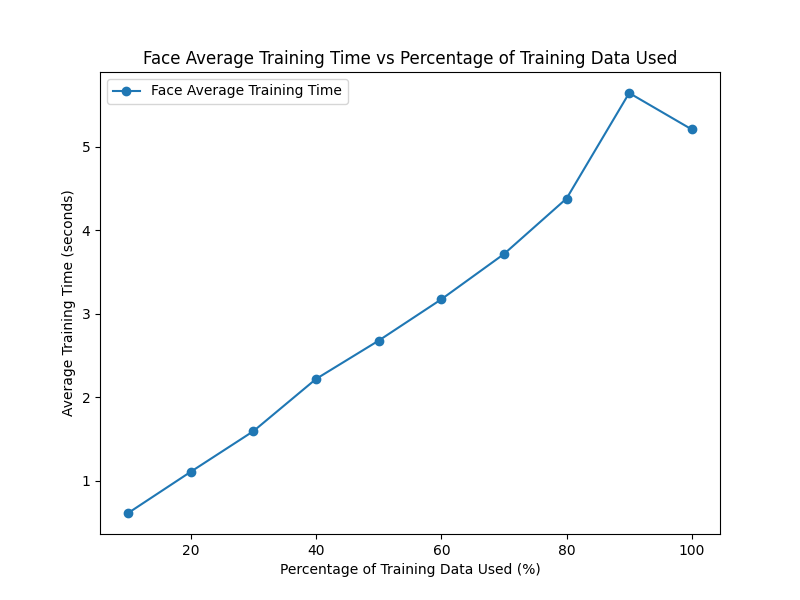
\includegraphics[width=.75\textwidth]{report/report_figures/pytorch_face_time.png}
\end{figure}
\begin{figure}[H]
    \centering
    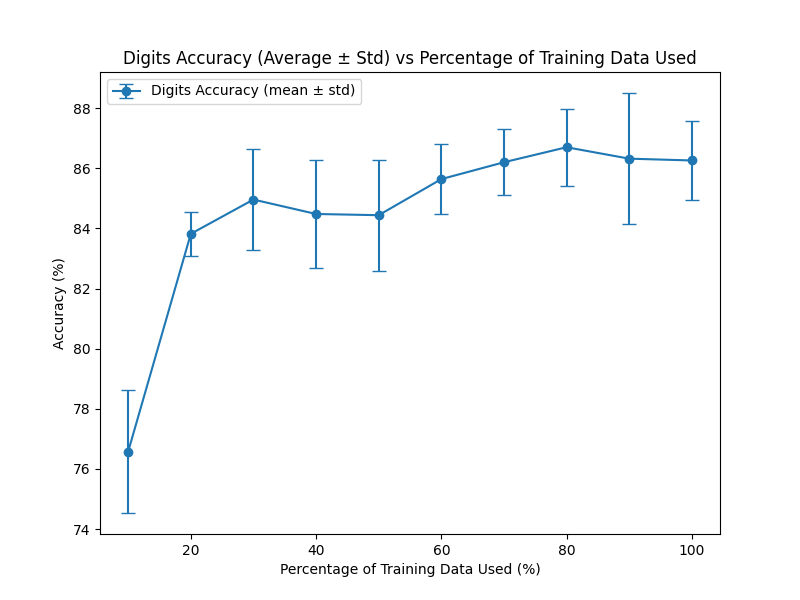
\includegraphics[width=.75\textwidth]{report/report_figures/pytorch_digits_acc.png}
\end{figure}
\begin{figure}[H]
    \centering
    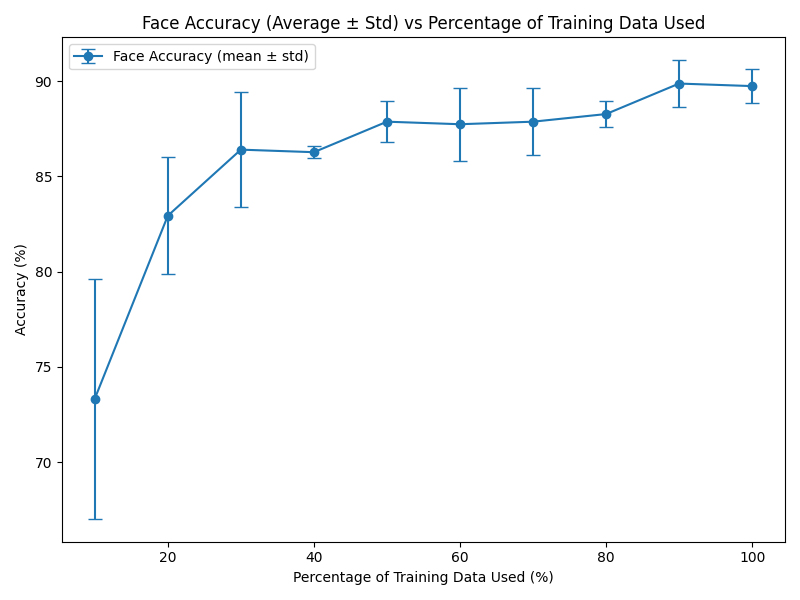
\includegraphics[width=.75\textwidth]{report/report_figures/pytorch_face_acc.png}
\end{figure}
\begin{figure}[H]
    \centering
    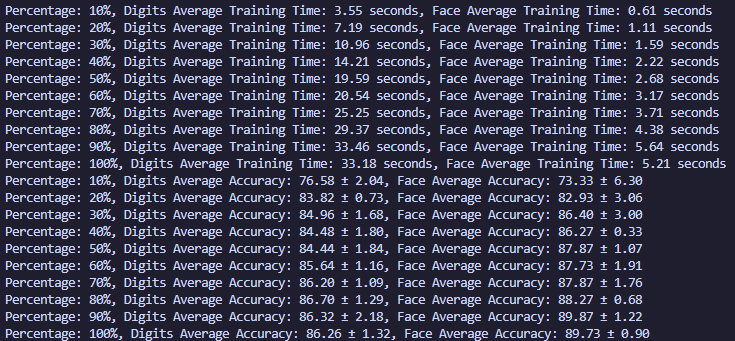
\includegraphics[width=.75 \textwidth]{report/report_figures/pytorch_output_log.png}
\end{figure}

\noindent Based on the average training time plots and output logs, the training time linearly increases with the percentage of training data used. This is expected as training on more data requires more computations. Also, the training for the digits dataset takes longer than the face dataset for the same percentage, which makes sense since there is more data for the digits dataset.

\noindent Based on the average test accuracy plots and output logs, the test accuracy generally increases with the percentage of training data used. For the digits dataset, the test accuracy increases but then begins to plateau around 80\%-100\%. The face dataset's test accuracy also increases, but then plateaus around 90\%-100\%. The standard deviation in accuracy generally stays between 1 and 2 for the digits dataset. For the face dataset, the standard deviation starts large and then quickly decreases, indicating the accuracy is becoming more consistent with more data. The face detection task achieves slightly higher accuracy than the digit recognition task past 20\%.


\section*{Results/Discussion}
Overall, we achieved good test average accuracies on both datasets with all three methods. Using 100\% of the training data, the lowest accuracy was 81.68\% on the digits dataset using perception, and the highest accuracy was 90.67\% on the face dataset using the manual three-layer neural network. We should note that the neural networks differed in the number of layers, number of epochs, and initialization of the weights as we sought to deal with the vanishing gradient issue. Thus all differences in results should be taken with this in mind. In general, we observed that the test accuracy does improve with more data, but up to a certain point. Often, once around 50\%-70\% of the data was used, the accuracy would start to plateau or decrease in one case. In general, the standard deviation would decrease as more training data was used, showing more consistent training. For the digits dataset, the standard deviation would decrease slightly and then stay within a certain range. The face dataset would start with a large standard deviation and then usually decrease as more data was used. In terms of training time, we observed that the training time was generally proportional to the percentage of training data used. This is expected as usually the more data used, the more computations are performed, requiring more time. In terms of the methods, we noticed the Perceptron was fastest, then the Pytorch neural network, and then the manual neural network. This was as expected since the Perceptron is very simple, Pytorch has a lot of built-in optimization, and our neural network used many more epochs and also did not have the same optimizations.

\section*{Conclusion/Lessons Learned}
This project taught us a lot about machine learning/deep learning and how to conduct experiments. We learned about the tradeoff between the amount of training data used and the accuracy. More training data does not always result in better accuracy. We also learned the importance of picking the right hyperparameters like learning rate, activation function, weight initialization, and size of hidden layers. We also gained experience writing a neural network from scratch and writing one using libraries, which was much easier to implement. We also learned the value of implementing things in parallel. When implementing our manual neural network, we implemented it by doing 
the forward pass of each training point in the batch individually, which was very slow.
We could have instead done the whole batch at once with matrix operations. Finally, we learned about the complexity of even a small neural network.
\end{document}